\chapter{系统需求分析}

本章主要围绕基于 MIL-STD-6016 的战术数据链信息标准数据库及其应用平台,分析系统的整体需求,明确功能性与非功能性要求,以便为后续系统设计与实现提供依据。

战术数据链作为现代联合作战的核心通信手段,其信息标准数据库的建设对于提升作战效能、增强系统互操作性具有重要意义。随着网络中心战概念的深入发展和多域作战需求的不断增长,传统的战术数据链系统面临着数据管理复杂、标准版本多样、跨链路互操作困难等挑战。因此,构建一个统一、高效、可扩展的战术数据链信息标准数据库系统,已成为当前军事信息化建设的重要任务。

本章将从系统需求分析的角度,全面阐述基于MIL-STD-6016标准的战术数据链信息标准数据库系统的功能需求、非功能性需求、数据特征与处理需求以及用户角色与交互需求。通过对这些需求的深入分析,为后续的系统架构设计、数据库建模、前后端开发以及系统集成测试提供明确的技术指导和约束条件。

\section{功能需求}

根据前期调研和标准分析,结合实际应用场景,系统需要实现以下核心功能:

\subsection{数据特征与处理需求}
战术数据链消息具有与传统业务数据不同的特性,其处理需求也更为复杂。为保证数据库的适用性与系统的实用性,需从数据来源、结构特征、处理方式与存储管理等角度加以分析\cite{baek2016_jsac}。

系统数据主要来源于 {MIL-STD-6016}、{MIL-STD-3011}、{STANAG-5516} 等标准文档,并结合 {MAVLink}、{NMEA-0183}、{ARINC-429} 等协议数据。数据类型主要包括:\textbf{标准消息数据}:J 系列报文(J2.0、J3.0、J7.0、J12.0等)及其字段定义;\textbf{语义概念数据}:基于CDM四层法的概念库和字段映射关系;\textbf{多格式文档数据}:PDF、XML、JSON、CSV等格式的标准文档和配置文件;\textbf{跨协议转换数据}:不同协议间的消息转换和映射规则。

表\ref{table_data_features}详细展示了战术数据链数据特征与处理需求的对应关系,该表从数据类型、结构特点、处理需求和存储实体四个维度进行了系统性的分析。标准消息数据具有多字段和比特位结构特点,需要系统具备报文解析和完整性校验能力,对应的存储实体包括消息表和字段表。语义概念数据具有概念层次和同义映射特点,需要系统支持概念绑定和语义一致性维护,对应的存储实体包括概念表和绑定表。多格式文档数据具有格式多样和结构复杂特点,需要系统支持多格式解析和智能识别,对应的存储实体包括文档表和解析结果表。跨协议转换数据具有格式差异和协议适配特点,需要系统支持格式转换和协议映射,对应的存储实体包括映射表和转换规则表。这种分类设计为系统的数据处理能力规划提供了清晰的指导。

\begin{table}[!htb]
    \caption{战术数据链数据特征与处理需求概览}
    \label{table_data_features}
    \centering
    \adjustbox{width=0.9\textwidth,center}{%
    \begin{tabular}{lccc}
        \hline
        \textbf{数据类型} & \textbf{结构特点} & \textbf{处理需求} & \textbf{存储实体} \\
        \hline
        标准消息数据 & 多字段/比特位 & 报文解析、完整性校验 & 消息表、字段表 \\
        语义概念数据 & 概念层次/同义映射 & 概念绑定、语义一致性 & 概念表、绑定表 \\
        多格式文档数据 & 格式多样/结构复杂 & 多格式解析、智能识别 & 文档表、解析结果表 \\
        跨协议转换数据 & 格式差异/协议适配 & 格式转换、协议映射 & 映射表、转换规则表 \\
        \hline
    \end{tabular}%
    }
\end{table}

战术数据链消息具有以下显著特征\cite{jiang2019_sensors}:\textbf{结构复杂}:消息由多个字段组成,字段具备不同的起始位、结束位与位长,需严格遵循标准规范;\textbf{语义多样}:同一字段在不同上下文下可能代表不同含义,需通过语义绑定提升一致性;\textbf{实时性要求高}:消息常用于态势共享和火力协调,必须在低延迟条件下完成解析与处理;\textbf{异构性强}:来自不同链路或版本的消息在格式与语义上存在差异,需要跨标准的映射与转换。

针对上述特征,系统在数据处理方面需满足以下要求\cite{hegarty_1997_nav_interference}:\textbf{消息解析与校验}:自动完成报文解析、字段提取与完整性校验;\textbf{语义绑定与转换}:建立字段与语义概念的映射关系,支持跨链协议的数据互操作;\textbf{批量处理}:支持大规模数据的批量导入、导出与清洗,提高建库与实验效率;\textbf{实时处理}:支持高速消息流的实时解析与存储,满足仿真平台和作战任务的即时需求。

系统需保证战术数据链数据库的高效存储与可维护性\cite{schnaufer_mcgraw_1997_waas}:\textbf{模式化存储}:采用关系数据库模式定义消息、字段、概念等实体,保证数据一致性;\textbf{分布式存储支持}:在高并发和大规模数据情况下,支持分片存储与负载均衡;\textbf{版本与追踪}:对不同版本标准及消息更新建立版本控制,便于历史追溯与对比;\textbf{安全与备份}:提供加密存储与多节点备份机制,保证敏感数据的安全性和可恢复性。

图\ref{fig_system_architecture}展示了基于MIL-STD-6016的战术数据链信息标准数据库系统的整体架构。系统采用分层架构设计,包括前端用户界面层、API网关层、业务逻辑层、数据处理层和数据存储层。前端层提供统一文档处理与语义互操作平台,支持消息处理、文件处理、概念管理、映射管理和系统概览等功能模块。API网关层整合了多个API接口,包括统一API(/api/v2)、CDM互操作API(/api/cdm)、语义互操作API(/api/semantic)等。业务逻辑层包含PDF处理服务、MQTT处理服务、语义互操作系统、CDM四层法系统和通用导入系统。数据处理层负责消息解析、字段提取、语义绑定和数据校验。数据存储层采用关系数据库模式,支持消息表、字段表、概念表、映射表等核心实体。

\begin{figure}[H]
    \centering
    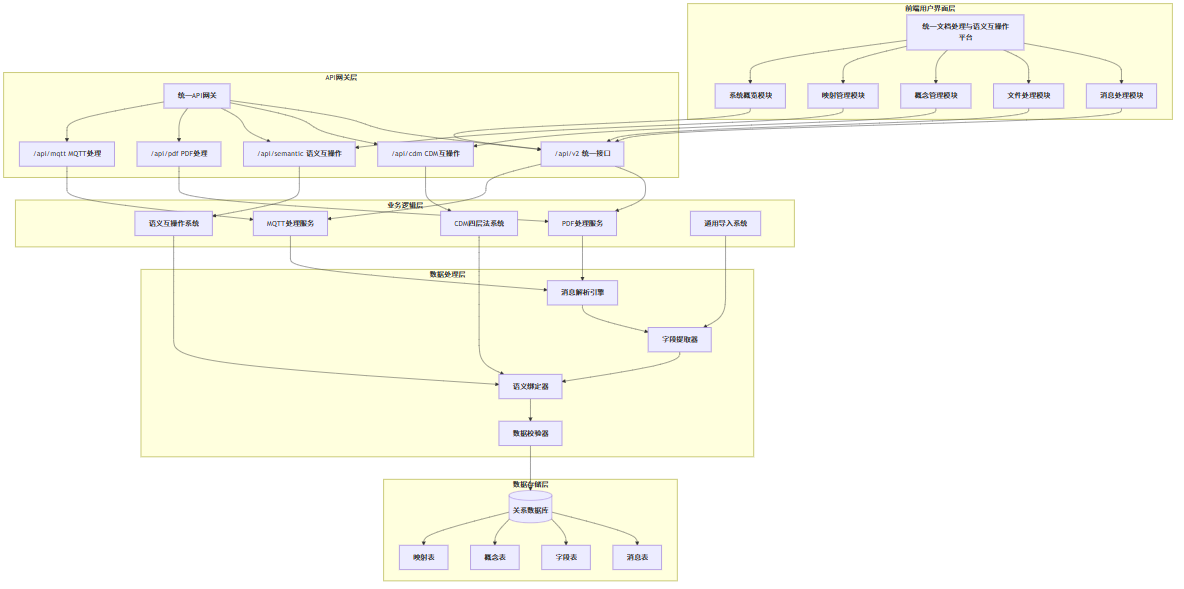
\includegraphics[width=0.85\textwidth,height=0.7\textheight,keepaspectratio]{chapters/fig-0/system_architecture.png}
    \caption{系统整体架构图}
    \label{fig_system_architecture}
\end{figure}

\subsection{标准消息管理}
战术数据链信息标准数据库系统需要支持多种消息标准的统一管理\cite{CurtissWright_TCG_HUNTR_2020}。根据实际应用需求分析,系统应具备以下核心能力:

(1)多标准消息支持:系统需要同时支持MIL-STD-6016的J系列消息(J2.0、J3.0、J7.0、J12.0等)、MAVLink的飞行器通信消息(HEARTBEAT、ATTITUDE、POSITION等)、NMEA-0183的导航消息(GGA、RMC、VTG等)等多种标准。每种消息标准都有其特定的格式、语义和应用场景,系统需要能够完整地存储和管理这些消息的定义信息,包括消息的基本属性、消息结构以及消息的语义信息。

表\ref{table_supported_standards}详细列出了系统支持的主要标准和协议。系统支持6个主要标准,包括3个军事标准(MIL-STD-6016、MIL-STD-3011、STANAG-5516)和3个通用协议(MAVLink、NMEA-0183、ARINC-429)。每个标准都有多个版本,支持不同类型的消息。MIL-STD-6016支持J系列消息,包括J2.0、J3.0、J7.0、J12.0等;MAVLink支持飞行器通信消息,包括HEARTBEAT、ATTITUDE、POSITION等;NMEA-0183支持导航消息,包括GGA、RMC、VTG等。这种多标准支持能力确保了系统能够处理来自不同数据链和协议的消息数据。

\begin{table}[!htb]
    \caption{系统支持的标准和协议}
    \label{table_supported_standards}
    \centering
    \adjustbox{width=0.9\textwidth,center}{%
    \begin{tabular}{lccc}
        \hline
        \textbf{标准名称} & \textbf{描述} & \textbf{版本} & \textbf{主要消息类型} \\
        \hline
        MIL-STD-6016 & 美军标准6016 - 战术数据链消息标准 & A, B, C & J2.0, J3.0, J7.0, J12.0, J13.0 \\
        MIL-STD-3011 & 美军标准3011 - 联合战术信息分发系统 & A, B & J2.0, J2.2, J3.0, J3.1, J3.3 \\
        STANAG-5516 & 北约标准5516 - 战术数据交换 & 1, 2, 3 & J2.0, J3.0, J7.0, J12.0 \\
        MAVLink & 微型飞行器通信协议 & 1.0, 2.0 & HEARTBEAT, ATTITUDE, POSITION, GPS\_RAW\_INT \\
        NMEA-0183 & 海洋电子设备数据格式 & 2.0, 2.1, 2.2, 2.3 & GGA, RMC, VTG, GLL, GSA \\
        ARINC-429 & 航空电子设备数字信息传输 & 15, 16, 17 & A429, A629 \\
        \hline
    \end{tabular}%
    }
\end{table}

(2)消息录入与维护:考虑到标准文档的复杂性和多样性,系统需要支持多种数据录入方式。传统的逐条录入方式效率低下,无法满足大规模标准文档的处理需求。系统需要提供基于PDF文档的自动化解析功能,能够从标准文档中自动提取消息定义信息,并支持CSV、Excel、XML、JSON等多种格式的批量导入和单个录入两种方式。

(3)消息字段管理:J系列消息的字段结构复杂,包含字段名称、起始位置、结束位置、位长度、描述信息等多个属性。系统需要能够处理这种复杂的字段结构,并建立字段与消息之间的关联关系。同时,系统需要支持字段的层次化组织,如字段组、子字段等,以便于更好地管理和理解消息结构。

(4)版本管理与兼容性:由于战术数据链标准会定期更新,系统需要能够管理不同版本的标准定义。系统需要支持版本对比功能,能够显示不同版本之间的差异,包括新增的消息、修改的字段、删除的内容等。这对于标准演进研究和系统升级具有重要意义。

(5)查询与检索:为提高查询效率,系统需要对消息进行多维度分类,包括按消息功能、按优先级、按使用频率等。系统需要建立高效的索引机制,支持基于消息号、字段名、时间戳等关键属性的快速检索。此外,系统还需要提供模糊查询和智能推荐功能,帮助用户快速定位所需消息。


\subsection{字段与语义概念绑定}
为提升消息语义一致性,系统需要支持字段与语义概念的绑定\cite{Chelton_Link16_Antennas_2022}。根据实际应用需求分析,系统应具备以下核心能力:

(1)语义概念库构建:系统需要建立统一的语义概念库,包含战术数据链领域中的核心概念,如平台标识、位置信息、时间信息、任务状态等。每个语义概念都应具有明确的定义、属性描述和使用规则,支持概念的层次化组织和继承关系。

(2)字段绑定机制:系统需要支持自动绑定和手动绑定两种方式。自动绑定基于字段名称、数据类型、取值范围等特征进行匹配,能够快速建立初步的绑定关系。手动绑定允许专家用户根据领域知识进行精确的绑定操作,确保绑定的准确性和完整性。

(3)置信度管理:系统需要为每个字段-概念绑定关系分配置信度值,反映绑定的可靠程度。置信度可以通过字段名称相似度、数据类型匹配度、专家验证结果等因素计算,并提供置信度阈值设置功能,允许用户根据应用需求调整绑定标准。

(4)绑定关系可视化:系统需要提供多种可视化方式,如概念层次图、字段映射矩阵、绑定关系网络图等,支持交互式操作,允许用户查看详细信息、修改绑定关系、导出绑定结果。

(5)动态绑定更新:考虑到战术数据链标准的不断演进,系统需要支持语义绑定的动态更新,当标准版本更新或新增消息类型时,能够自动检测需要重新绑定的字段,并提供批量更新功能。

\subsection{多链路互操作支持}
考虑到战术数据链存在多标准并行的情况,系统需要具备跨链路的互操作支持功能\cite{AFCEA_Link16_Improvements_2022}。根据实际应用需求分析,系统应具备以下核心能力:

(1)CDM四层法架构:系统需要采用CDM(Common Data Model)四层法架构实现多协议互操作。概念层定义统一的语义概念库,包含作战实体、态势要素、指挥关系等核心概念;映射层通过声明式规则定义协议间的字段映射关系;转换层实现具体的消息转换逻辑;运行层提供协议中介和转换引擎。系统支持MIL-STD-6016、MAVLink、MQTT、NMEA-0183等协议的互操作转换,这种分层架构确保系统的可扩展性和可维护性。
图\ref{fig_cdm_architecture}展示了CDM四层法架构,包括语义层(统一概念库)、映射层(YAML配置规则)、校验层(一致性验证)和运行层(转换引擎),实现多协议间的语义互操作和实时转换。

\begin{figure}[H]
    \centering
    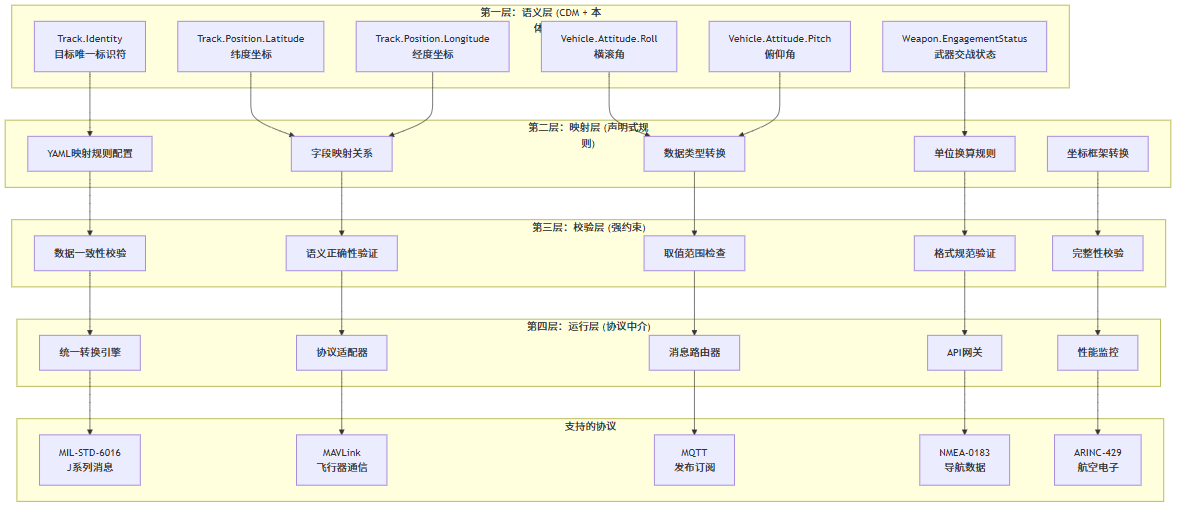
\includegraphics[width=0.8\textwidth,height=0.5\textheight,keepaspectratio]{chapters/fig-0/cdm_architecture.png}
    \caption{CDM四层法架构图}
    \label{fig_cdm_architecture}
\end{figure}

(2)智能消息转换引擎:系统需要实现基于规则和机器学习的智能转换引擎,能够自动处理协议间的语法差异、语义差异和时序差异。转换引擎需要支持多种转换策略,包括精确匹配、模糊匹配、语义推理等,并提供转换质量评估和置信度评分机制。系统还需要支持转换规则的动态更新和版本管理,以适应协议演进的需求。

(3)统一API网关:系统需要提供统一的API网关,支持多种协议的消息转换和路由。网关需要集成CDM四层法和语义互操作两种处理方式,能够根据源协议和目标协议自动选择最优的转换策略。网关还需要提供实时监控、性能分析、错误处理等功能,确保系统的高可用性和稳定性。表\ref{table_api_interfaces}列出了系统提供的5个主要API接口及其功能,通过RESTful架构设计为前端界面和外部系统提供标准化数据交换接口。

\begin{table}[!htb]
    \caption{系统API接口功能表}
    \label{table_api_interfaces}
    \centering
    \adjustbox{width=0.9\textwidth,center}{%
    \begin{tabular}{lccc}
        \hline
        \textbf{API接口} & \textbf{主要功能} & \textbf{支持格式} & \textbf{应用场景} \\
        \hline
        /api/v2 & 消息转换、概念管理、映射管理、系统统计 & JSON, XML & 统一文档处理与语义互操作 \\
        /api/cdm & CDM概念创建、映射规则管理、消息转换 & JSON, YAML & CDM四层法互操作处理 \\
        /api/semantic & 语义字段管理、消息映射、路由处理 & JSON, XML & 语义互操作系统 \\
        /api/pdf & PDF文档解析、表格提取、数据处理 & PDF, JSON & MIL-STD-6016文档处理 \\
        /api/mqtt & MQTT消息处理、协议转换、数据路由 & JSON, MQTT & MQTT协议消息处理 \\
        \hline
    \end{tabular}%
    }
\end{table}

(4)协议适配支持:系统需要支持MIL-STD-6016、MAVLink、MQTT、NMEA-0183、ARINC-429等多种协议的消息对接,能够处理不同协议间的消息格式差异、语义差异和时序差异。通过声明式映射规则和版本治理机制,系统需要能够灵活应对协议演进和标准更新。


\subsection{数据库操作与维护}
战术数据链信息标准数据库系统需要处理大量的结构化数据,包括消息定义、字段信息、语义绑定关系等,这些数据的准确性和完整性直接影响系统的功能实现和用户体验。因此,系统必须提供完善的数据导入导出与版本管理功能,支持CSV、Excel、XML、JSON、SQL等多种格式的批量数据处理。导入功能需要具备数据验证和错误处理能力,能够自动检测数据格式错误、重复记录、缺失字段等问题,并提供详细的错误报告和修复建议。导出功能需要支持灵活的数据筛选和格式化选项,允许用户根据需要选择导出内容和格式。同时,系统需要实现完整的数据版本控制机制,记录每次数据变更的详细信息,包括变更时间、变更用户、变更内容等,支持数据回滚功能和审计追踪功能,确保数据完整性和可追溯性。

为确保系统长期稳定运行和数据安全,系统需要实现基于角色的访问控制(RBAC)和实时性能监控机制。权限管理需要为不同用户分配不同的权限级别,包括数据访问权限、操作权限、管理权限等,确保用户只能访问和操作其权限范围内的数据和功能。系统还需要提供细粒度的权限控制,支持字段级别的访问控制,保护敏感信息的安全。此外,系统需要提供实时的性能监控功能,包括数据库连接数、查询响应时间、系统资源使用率等关键指标,支持告警机制和性能优化建议,帮助管理员识别和解决性能瓶颈问题,确保系统的高可用性和稳定性\cite{Lekkakos_2008}。

\subsection{前端交互与可视化}
战术数据链信息标准数据库系统面向的用户群体包括系统管理员、作战指挥员、研发人员等,这些用户具有不同的技术背景和使用需求,因此前端系统需要提供直观、易用、功能丰富的用户界面。系统应提供统一文档处理与语义互操作平台,包含消息处理、文件处理、概念管理、映射管理、系统概览等核心功能模块,支持用户通过消息号、字段名、J系列类别、时间范围等多种条件进行精确查询,并支持查询条件的保存和重用,允许用户创建常用的查询模板。

数据展示应支持多种方式,包括表格、图表、关系图等,其中表格展示应支持排序、筛选、分页等功能,并提供数据导出能力,图表展示应支持多种图表类型,如柱状图、饼图、折线图等,帮助用户直观地理解数据分布和趋势。同时,系统还应提供智能搜索功能,支持模糊匹配和语义搜索,帮助用户快速定位所需信息。

为确保良好的用户体验和系统可用性,前端系统需要支持交互式操作和响应式设计。系统应支持拖拽、点击、缩放等交互操作,允许用户通过直观的手势操作来浏览和操作数据,并提供上下文菜单、快捷键等便捷操作方式,提高用户的操作效率。同时,系统应支持个性化设置,允许用户自定义界面布局、颜色主题、显示选项等。此外,系统应支持桌面端、平板端、移动端等多种设备,确保在不同屏幕尺寸下都能提供良好的用户体验,响应式设计应能够自动适应屏幕尺寸,调整界面布局和功能显示,确保系统的可用性和易用性\cite{Ho_2008}。

系统需针对不同用户提供差异化的交互模式\cite{reid_2018_nav_leo}:

(1)\textbf{图形化交互}:前端界面提供消息检索、态势展示和跨链协议映射的可视化操作,支持CDM互操作接口、语义互操作接口和统一处理器接口,降低使用门槛,如图\ref{fig_usecase_frontend}所示。
% ================= 新增:用例图 =================
\begin{figure}[H]
    \centering
    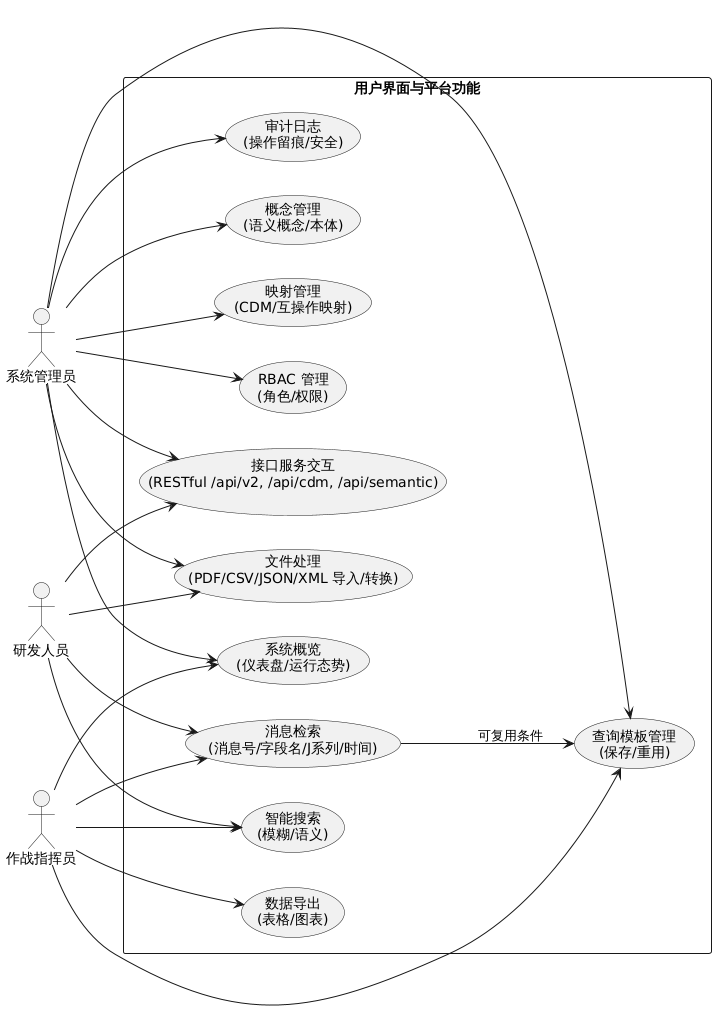
\includegraphics[width=0.8\textwidth,height=0.5\textheight,keepaspectratio]{chapters/fig-0/usecase_frontend.png}
    \caption{前端交互用例图(角色与功能关系)}
    \label{fig_usecase_frontend}
  \end{figure}
(2)\textbf{命令行接口}:为研发与仿真人员提供批处理与脚本化调用,支持大规模数据处理与自动化测试。

(3)\textbf{接口服务交互}:通过 RESTful API 与外部仿真平台或作战系统对接,支持标准化协议调用和跨域互操作,提供/api/v2、/api/cdm、/api/semantic等统一API接口,如图\ref{fig_component_frontend} 所示。



% ================= 新增:组件图 =================
\begin{figure}[H]
  \centering
  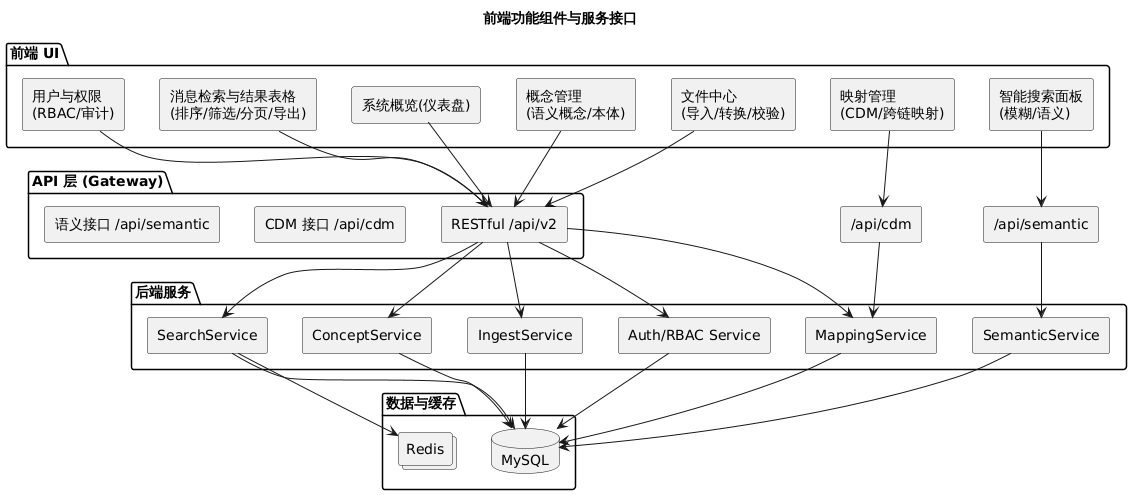
\includegraphics[width=0.8\textwidth,height=0.5\textheight,keepaspectratio]{chapters/fig-0/component_frontend.png}
  \caption{前端功能组件与服务接口关系图}
  \label{fig_component_frontend}
\end{figure}


\subsection{仿真与验证接口}
战术数据链系统的验证和测试需要大量的仿真数据支持,而仿真平台则需要真实的消息定义和格式规范来生成准确的测试数据,因此系统必须提供完善的仿真与验证接口。系统应提供标准化的RESTful API接口,支持仿真平台进行数据查询、消息生成、结果验证等操作,API接口应遵循REST架构原则,使用标准的HTTP方法和状态码,确保接口的易用性和可维护性。同时,系统应支持多种标准化的消息输出格式,包括JSON、XML、YAML等,以满足不同仿真平台的格式需求,消息格式应包含完整的消息定义信息,包括消息结构、字段定义、语义信息等,确保仿真平台能够准确理解和处理消息数据。

为确保系统验证能力的完整性和可靠性,系统需要具备消息生成与回放功能以及仿真数据管理能力。消息生成功能应能够根据消息定义自动生成测试消息,支持不同场景和条件的消息生成,并支持参数化配置,允许用户设置消息类型、字段值、时间戳等参数。消息回放功能应能够重现历史消息流,支持性能测试和兼容性验证。此外,系统应提供仿真数据的存储、管理和检索功能,支持大量仿真数据的快速访问和处理,包括数据版本控制、数据质量检查、数据统计分析等功能,确保仿真数据的准确性和可用性,为大规模仿真测试提供可靠的数据基础\cite{Kao_2008}。
\section{系统非功能性需求分析}

战术数据链数据库及应用平台作为支撑作战指挥的关键信息系统,除了满足功能性需求外,还必须具备良好的非功能性特征,包括性能、安全性、可扩展性等方面的要求,以确保系统在复杂作战环境下的稳定运行和长期发展\cite{Kagioglidis_2009}。

\subsection{性能需求}
系统需要保证在多用户同时访问的情况下维持较低的响应时间,普通查询请求的平均响应时间应不超过2秒,支持消息解析与字段检索的快速响应,以适应实时态势更新的需求\cite{Kee_2008,baek2016_adhoc,baek2019_jsyst_timemirror}。为满足上述性能要求,系统需要实现缓存机制,包括Redis缓存和查询结果缓存,对于频繁访问的消息类型和字段定义实现预加载策略,同时建立数据库索引支持多条件组合查询的快速执行。

系统需要具备较高的数据吞吐能力,支持批量数据导入导出操作,仿真接口可持续处理消息流,实现消息实时生成与回放\cite{lee2018_jsyst,Spyridis_2010,Kopp_Throughput_Enhanced_JTIDS_2006,Juarez_2025}。同时,考虑到战术环境的复杂性,系统需具备基本的可靠性与容错能力,数据库采用备份与日志恢复机制,保证数据在异常情况下不丢失,系统应支持事务一致性,确保消息存储与语义绑定过程的完整性\cite{Koromilas_2009,EverythingRF_STT}。

\subsection{安全性需求}
战术数据链系统涉及敏感作战信息,安全性需求至关重要。系统必须在数据存储、传输与访问控制等方面提供基本的安全保障,以确保信息不被篡改、泄露或非法利用\cite{Collins_TTNT_immersion_2020}。系统应在数据存储和传输过程中采用加密技术,数据库层面应对核心字段进行加密存储,系统接口需采用基于TLS/SSL的安全传输协议,防止中间人攻击,消息交互采用密钥管理机制,定期更新密钥,防止密钥泄露\cite{Euromids_2025_contract}。

为防止非法访问与误操作,系统需建立访问控制机制,提供基于角色的访问控制(RBAC),不同用户角色具备不同权限范围,对数据库的读写操作需进行身份认证与授权,提供日志审计功能,记录用户操作轨迹,便于事后追溯\cite{GovConWire_Euromids_2025}。系统应提供数据校验与完整性验证机制(如哈希校验),在通信中断或错误发生时,系统可通过重传机制与数据恢复策略保证一致性\cite{musumeci_2014_ietrsn_pulseblank,borio_2013_ietspr_pulseblanking,houdzoumis2009_jn,wu_2016_taes_dme_wp,huo_2015_ieeecl_meb,huo_2015_comex_mixed_interference,mitch_2016_nav_chirp_geolocation,vandermerwe_2023_nav_mpanf}。

\subsection{可扩展性需求}
随着战术数据链标准的不断更新与作战样式的演进,系统必须具备良好的可扩展性,以适应未来的技术升级与功能扩展需求\cite{CJCS_Manuals_Library}。系统应能够适配不同版本的Link 16标准以及相关NATO STANAG的扩展,数据库设计应采用模块化和可扩展的模式,支持新增消息类型、字段及语义映射,在MIL-STD-6020和STANAG 5602等互操作标准演进过程中,系统应可快速接入新接口与协议\cite{CJCS_Instructions_Library,ASSIST_3011_2023}。

在多链路并行和跨域作战背景下,系统需支持不同数据链协议的融合,除Link 16外,系统架构应预留与TTNT、JREAP、未来新型数据链的扩展接口,提供协议适配层,保证不同链路间的数据结构映射与消息语义转换\cite{ASSIST_6020_2025,qin2013_gpssol}。为支撑未来规模化应用和复杂环境下的运行,系统整体架构需具备扩展能力,后端采用微服务架构,支持按需部署,前端应支持模块化扩展,便于快速集成新型可视化与交互模块,数据库采用可扩展架构,支持数据分片与多节点扩展\cite{fried_loeliger1979_navigation}。系统应提供标准化接口,以支持与外部系统的互联互通,采用RESTful API协议,方便外部仿真平台、指挥信息系统接入,提供标准化数据交换格式(如JSON、XML),便于与异构系统交互,具备开放API文档与开发者支持,方便后续功能拓展与二次开发\cite{baruffa2013_jsps}。
